%!TEX program = xelatex
%!TEX output_directory = build
\documentclass[UTF8,11pt,a4paper,fontset=fandol,scheme=plain]{ctexart}
% Layout adapted from the user's modular PhD proposal projects.
% MAIN ADJUSTMENT POINTS: geometry, setstretch, parindent, titlespacing, captions.
\usepackage[a4paper,margin=2.54cm,headheight=15pt,headsep=0.7cm,footskip=0.9cm]{geometry}
% XeLaTeX + ctexart: Fandol fonts ship with TeX Live; no macOS-only fonts.
\setmainfont{texgyretermes-regular.otf}[BoldFont=texgyretermes-bold.otf,ItalicFont=texgyretermes-italic.otf,BoldItalicFont=texgyretermes-bolditalic.otf]
\setsansfont{texgyreheros-regular.otf}[BoldFont=texgyreheros-bold.otf,ItalicFont=texgyreheros-italic.otf,BoldItalicFont=texgyreheros-bolditalic.otf]
\renewcommand{\contentsname}{目录}
\renewcommand{\figurename}{图}
\renewcommand{\tablename}{表}
\usepackage{setspace,microtype,xcolor,graphicx}
\usepackage{enumitem,titlesec,fancyhdr,caption,placeins,needspace}
\usepackage[round,authoryear]{natbib}
\usepackage{xurl}
\usepackage{array,tabularx,longtable}
% Academic tables: white background, black text, 0.4pt rules.
\newcolumntype{L}[1]{>{\raggedright\arraybackslash}p{#1}}
\newcolumntype{Y}{>{\raggedright\arraybackslash}X}
\newcommand{\ReportTableSetup}{%
  \small\setstretch{1.15}%
  \setlength{\tabcolsep}{6pt}%
  \setlength{\arrayrulewidth}{0.4pt}%
  \renewcommand{\arraystretch}{1.25}%
  \color{black}}

\usepackage[colorlinks=true,linkcolor=black,citecolor=black,urlcolor=FinTaxBlue,bookmarksnumbered=true]{hyperref}
\definecolor{FinTaxBlue}{HTML}{3952EF}
\definecolor{FinTaxInk}{HTML}{172033}
\definecolor{FinTaxGray}{HTML}{636B78}
\setstretch{1.3}
\setlength{\parindent}{2em}
\setlength{\parskip}{0pt}
\setlength{\emergencystretch}{2em}
\setlist{nosep,leftmargin=0.5in,topsep=4pt,itemsep=3pt}
\setcounter{secnumdepth}{2}
\setcounter{tocdepth}{2}
\titleformat{\section}{\large\bfseries\color{FinTaxInk}}{\thesection.}{0.5em}{}
\titleformat{\subsection}{\normalsize\bfseries}{\thesubsection}{0.5em}{}
\titlespacing*{\section}{0pt}{18pt plus 2pt minus 2pt}{8pt}
\titlespacing*{\subsection}{0pt}{14pt plus 2pt minus 2pt}{6pt}
\captionsetup{font=small,labelfont=bf,labelsep=period,justification=raggedright,singlelinecheck=false,skip=7pt}
\pagestyle{fancy}
\fancyhf{}
\fancyhead[L]{\footnotesize\sffamily\textbf{FinTax}\quad\color{FinTaxGray}研究报告}
\fancyhead[R]{\footnotesize\color{FinTaxGray}\ReportShortTitle}
\fancyfoot[L]{\footnotesize\color{FinTaxGray}\ReportDate\quad |\quad fintax.tech}
\fancyfoot[R]{\footnotesize\thepage}
\renewcommand{\headrulewidth}{0.4pt}
\renewcommand{\footrulewidth}{0pt}
\fancypagestyle{plain}{\fancyhf{}\fancyfoot[R]{\footnotesize\thepage}\renewcommand{\headrulewidth}{0pt}}
\urlstyle{same}
\widowpenalty=10000
\clubpenalty=10000
\raggedbottom
% Original map and screenshots; tables are editable files in tables/.
\newcommand{\ReportImage}[3]{%
  \begin{figure}[htbp]
  \centering
  \includegraphics[width=\linewidth,height=0.60\textheight,keepaspectratio]{assets/figure-#1.png}
  \captionsetup{type=#2}\caption{#3}
  \end{figure}}

% 报告信息集中在此处修改；排版参数位于 preamble.tex。
\newcommand{\ReportTitle}{加密矿企转型 AI 数据中心}
\newcommand{\ReportSubtitle}{美国各州税收优惠与关键考量}
\newcommand{\ReportShortTitle}{美国数据中心税收优惠}
\newcommand{\ReportDate}{2026年8月25日}
\newcommand{\ReportPublisher}{FinTax}
\newcommand{\ReportURL}{https://www.fintax.tech/reports/crypto-miners-pivot-to-ai-data-centers-u-s-state-tax-incentives-and-key-considerations}
\hypersetup{
  pdftitle={加密矿企转型 AI 数据中心：美国各州税收优惠与关键考量},
  pdfauthor={FinTax},
  pdfsubject={FinTax 研究报告（中文翻译排版初稿）},
  pdfkeywords={加密挖矿, AI 数据中心, 税收优惠, 得克萨斯州, 弗吉尼亚州, 佐治亚州},
  pdfdisplaydoctitle=true,
  pdflang={zh-CN}
}


\begin{document}
\hypersetup{pageanchor=false}
\begin{titlepage}
\thispagestyle{empty}
\noindent
\includegraphics[width=43mm]{assets/fintax-logo-lockup.pdf}
\vspace{27mm}

\noindent{\sffamily\small\bfseries\color{FinTaxBlue}研究报告}\par
\vspace{9mm}
\noindent{\raggedright\hyphenpenalty=10000\fontsize{29}{34}\selectfont\bfseries\color{FinTaxInk}\ReportTitle\par}
\vspace{7mm}
\noindent{\fontsize{18}{24}\selectfont\color{FinTaxInk}\ReportSubtitle\par}
\vspace{13mm}
\noindent{\large\ReportDate\par}
\vfill
\noindent{\bfseries\ReportPublisher}\par
\smallskip
\noindent 面向加密机构的财务与税务解决方案\par
\medskip
\noindent\href{https://www.fintax.tech}{www.fintax.tech}
\end{titlepage}

\pagenumbering{roman}
\hypersetup{pageanchor=true}
\tableofcontents
\vfill
\noindent\textbf{关于本中文版}\par
\noindent 本文依据 FinTax 于\ReportDate{}发布的英文报告翻译，为中文排版初稿。
保留原报告章节、数据和论述，三张表格改为可编辑的黑白线框表格，地图及申请表截图保留英文原图。
封面、目录、页码及来源说明为本 PDF 版本新增内容，政策表述保留原报告发表时的语境。\par
\medskip
\noindent\href{\ReportURL}{在 fintax.tech 阅读英文原文}
\clearpage
\pagenumbering{arabic}
\section{加密矿企正在转向 AI 数据中心}

自2024年以来，比特币减半周期、比特币价格回调及市场竞争加剧等因素共同作用，持续压缩加密矿企传统业务的利润空间。多家矿企宣布转向数据中心业务，希望将现有数字基础设施资产重新部署到快速增长的 AI 市场。

今年，数据中心转型进一步进入落地阶段。MARA 着手收购数据中心及已具备供电条件的场地，取得法国电力公司 EDF 旗下 Exaion 的控股权，并将数字基础设施确定为主要增长方向，计划逐步把现有矿场发展为 AI／高性能计算（HPC）园区。Riot 第二季度的数据中心收入达到2,320万美元，并与一家领先的前沿 AI 实验室签订为期20年的数据中心协议，在其 Rockdale 园区提供191兆瓦的关键 IT 容量。2026年2月，Cipher 从 Cipher Mining 更名为 Cipher Digital，将业务定位扩展至数据中心开发与运营。

在挖矿经济性承压的背景下，加密矿企必须重新评估每一兆瓦电力对应的成本与回报。过去用于挖矿的工业用地、电力基础设施和冷却系统，随着 AI 需求加速增长，可能产生更稳定且更具吸引力的收益。

一旦企业决定重新部署这些资产并进入相关市场，新一轮资本投入便随之开始。销售和使用税、财产税以及用电税等税务因素，可能直接影响转型的投资成本。

本文选取美国部分州，梳理数据中心税收优惠的现状及最新动向，并深入分析得克萨斯州、弗吉尼亚州和佐治亚州等重点辖区的资格门槛与实施路径，为转型中的矿企提供实务参考。

\FloatBarrier

\section{美国数据中心税收优惠：政策格局与近期变化}

美国的数据中心税收优惠主要由州和地方政府设立。对于加密矿企改造或新建数据中心的项目，州级税收优惠主要影响两个方面。

第一，建筑材料与设备采购。在数据中心改造过程中，矿企可能需要购入大量有形动产，包括服务器、电气设备和网络设备，以支持新的业务活动。这些采购可能触发销售和使用税，而部分州会在满足特定条件时提供免税待遇。

第二，数据中心的持续运营。矿企的数据中心竣工并投入使用后，土地、建筑和设备仍可能需要缴纳财产税，大量用电也可能涉及销售税、公用事业税或用电税。因此，部分州和地方政府会提供财产税减免、与电力相关的免税待遇或其他经济激励。

多年来，美国许多州通过税收优惠吸引数据中心投资。但到2026年，公众对数据中心基础设施的态度开始由支持转向反对，政策环境也出现明显变化。

得克萨斯州、弗吉尼亚州和佐治亚州等主要辖区的销售和使用税优惠，仍适用于符合条件的项目。与此同时，AI 数据中心快速扩张引发了对电价、水资源和当地居民负担的广泛关注，促使多个州暂停数据中心优惠，或考虑采取类似措施。自2026年夏季起，亚利桑那州对新的计算机数据中心税收减免申请实施为期三年的暂停受理措施；华盛顿州取消了服务器更换设备和翻新项目的销售和使用税优惠；路易斯安那州则提高了数据中心优惠的附加条件，包括要求数据中心企业承担其项目带来的全部新增电力需求。

这意味着，加密矿企在转型过程中仍可能获得税收优惠，但优惠的可获得性正变得更不确定。项目选址、是否需要新的免税资格认证、申请时点以及政策调整引入的新因素，都可能影响转型的实际税务成本。

% 依据英文版表1逐项翻译，数值与条件沿用原稿。
\begingroup
\ReportTableSetup
\begin{longtable}{|L{0.15\linewidth}|L{0.23\linewidth}|L{\dimexpr0.62\linewidth-6\tabcolsep-4\arrayrulewidth\relax}|}
\caption{各州数据中心税收优惠状态}\label{tab:state-incentives}\\
\hline
\textbf{州} & \textbf{当前状态} & \textbf{主要变化} \\ \hline
\endfirsthead
\caption[]{各州数据中心税收优惠状态（续）}\\
\hline
\textbf{州} & \textbf{当前状态} & \textbf{主要变化} \\ \hline
\endhead
亚利桑那州 & 暂停新申请 & 自2026年7月1日至2029年6月30日，亚利桑那州商务管理局不得受理新计算机数据中心的申请。 \\ \hline
俄亥俄州 & 暂停新申请 & 俄亥俄州税收抵免管理局已暂停审议新的数据中心税收豁免请求。 \\ \hline
伊利诺伊州 & 暂停新协议 & 自2026年7月1日起，该州停止处理数据中心激励计划的新申请。 \\ \hline
马萨诸塞州 & 暂停新申请 & 自2026年6月25日起，该州暂停受理合资格数据中心销售和使用税豁免申请。 \\ \hline
华盛顿州 & 缩小免税范围 & 自2026年7月1日起，服务器更换设备不再适用原有豁免；不再签发新的农村地区翻新证书，城市地区翻新项目也不再符合资格。 \\ \hline
弗吉尼亚州 & 仍可免税；新增用电税 & 销售和使用税豁免继续有效；自2026年7月1日至2028年6月30日，按每千瓦时0.011美元征收数据中心用电税。 \\ \hline
路易斯安那州 & 仍可免税；条件待定 & 2026年6月的一项行政命令要求，为数据中心销售税优惠建立电费缴纳者和社区保护框架，具体标准由相关主管部门制定中。 \\ \hline
得克萨斯州 & 仍可免税；政策变化风险较高 & 该州要求全面审查数据中心电网互联项目，并提出与立法机关合作，取消过时或不必要的数据中心优惠。 \\ \hline

\end{longtable}
\endgroup


\FloatBarrier

\section{各州比较：不同项目情景下的税务规划}

\subsection{得克萨斯州：临时销售和使用税豁免}

根据《得克萨斯州税法》第151.359条及151.3595条，得克萨斯州为符合条件的数据中心和符合条件的大型数据中心项目提供临时销售和使用税豁免。符合条件的数据中心在合资格采购中可免缴6.25\%的州销售和使用税，但仍须缴纳地方销售和使用税；免税期为10年或15年。对于符合条件的大型数据中心项目，合资格采购可在20年内同时免缴州和地方销售和使用税。

免税范围涵盖数据中心运营所必需且不可或缺的电力和设备，包括服务器、数据存储设备和网络连接设备。对于电力采购，通常需要开展主要用途研究，以区分应税和非应税用电，除非数据中心或项目符合适用的独立设施要求。

% 两类项目相同的共同要求合并展示，分别保留具体门槛。
\Needspace{0.60\textheight}
\begingroup
\ReportTableSetup
\begin{longtable}{|L{0.28\linewidth}|L{\dimexpr0.72\linewidth-4\tabcolsep-3\arrayrulewidth\relax}|}
\caption{资格要求}\label{tab:texas-eligibility}\\
\hline
\multicolumn{2}{|L{\dimexpr\linewidth-2\tabcolsep-2\arrayrulewidth\relax}|}{\textbf{共同要求（适用于两类项目）}} \\ \hline
\multicolumn{2}{|L{\dimexpr\linewidth-2\tabcolsep-2\arrayrulewidth\relax}|}{1. 持有或同时申请得克萨斯州销售或使用税许可证，或得克萨斯州直接缴税许可证；} \\ \hline
\multicolumn{2}{|L{\dimexpr\linewidth-2\tabcolsep-2\arrayrulewidth\relax}|}{2. 提交说明如何达到资本投入及就业创造要求的计划文件，并附拟议场地平面图或建筑示意图；} \\ \hline
\multicolumn{2}{|L{\dimexpr\linewidth-2\tabcolsep-2\arrayrulewidth\relax}|}{3. 位于得克萨斯州；} \\ \hline
\multicolumn{2}{|L{\dimexpr\linewidth-2\tabcolsep-2\arrayrulewidth\relax}|}{4. 专门新建或翻修，主要用于容纳服务器、相关设备及支持人员，以进行数据处理、存储和分发；} \\ \hline
\multicolumn{2}{|L{\dimexpr\linewidth-2\tabcolsep-2\arrayrulewidth\relax}|}{5. 具备不间断电源、发电机备用电源、完善的消防及防火系统，以及加强的实体安保措施，包括限制出入、视频监控和电子系统；} \\ \hline
\multicolumn{2}{|L{\dimexpr\linewidth-2\tabcolsep-2\arrayrulewidth\relax}|}{6. 不得主要供电信服务商用于提供电信服务；} \\ \hline
\multicolumn{2}{|L{\dimexpr\linewidth-2\tabcolsep-2\arrayrulewidth\relax}|}{7. 不受根据《税法》第313章限制数据中心财产评估价值的协议约束。} \\ \hline

\textbf{类型} & \textbf{具体要求} \\ \hline
符合条件的数据中心 &
1. 承诺在所在县创造至少20个合资格就业岗位；\par
2. 承诺在五年内投入或同意投入至少2亿美元资本；\par
3. 具有至少100,000平方英尺、供单一合资格使用者使用的建筑空间。
\\ \hline
符合条件的大型数据中心项目 &
1. 承诺在所在县创造至少40个合资格就业岗位；\par
2. 承诺在五年内投入或同意投入至少5亿美元资本；\par
3. 具有至少250,000平方英尺、供单一合资格使用者使用的建筑空间。
\\ \hline
\end{longtable}
\endgroup


可享受免税待遇的合资格数据中心，须具有至少100,000平方英尺、供单一合资格使用者使用的空间，在认证后五年内投入至少2亿美元资本，并创造至少20个合资格就业岗位。对于符合条件的大型数据中心项目，门槛提高至总面积至少250,000平方英尺、五年内资本投入至少5亿美元，以及至少40个合资格岗位。

实施要求明确允许数据中心设施为专门新建或翻修的设施。因此，现有矿场的改造不会仅因其原始用途而被排除在优惠范围之外。

为持续享受免税待遇，相关企业还必须遵守后续要求，包括履行适用的资本投入和合资格岗位承诺，向得克萨斯州审计长办公室提交规定报告，并完整保存免税采购记录，直至数据中心认证到期。审计长办公室会审查合规情况并开展审计；不符合要求的数据中心可能失去免税待遇，或被撤销认证。

\subsection{弗吉尼亚州：零售销售和使用税豁免与用电税}

《弗吉尼亚州法典》第58.1-609.3(18)条规定，符合条件的数据中心运营商及其租户购买或租赁合资格计算机设备和配套软件，可免缴零售销售和使用税（DCRSUT 豁免）。该豁免目前有效至2035年6月30日。如果数据中心满足特定资本投入及就业创造要求，可通过谅解备忘录（MOU）将豁免期延长至2040年或2050年。

合资格计算机设备包括服务器、路由器及数据存储设备，并明确涵盖支持免税设备运行的线缆、交换机、布线及类似物品。但与数据处理无关的一般建筑改良和固定设施，例如照明和围栏，不在豁免范围内；原本须缴纳零售销售和使用税、用于供电的燃料也不适用该豁免。

与得克萨斯州不同，一般地区的数据中心运营商及租户需要新增至少1.5亿美元资本投入。此外，数据中心须创造至少50个与数据中心运营或维护相关的就业岗位，每个岗位的薪酬至少达到当地通行年平均工资的150\%。在经济困难地区，法定门槛降低至7,000万美元资本投入，以及10个与运营或维护相关的岗位。

\ReportImage{3}{figure}{一般地区（灰色）与经济困难地区（蓝色）的分布；地名保留英文原图}

DCRSUT 豁免附有记录保存和报告要求。数据中心及其租户必须完整、准确地记录资本投入、新增岗位数量及其年平均工资、合资格计算机设备或配套软件支出，以及 DCRSUT 豁免的金额。数据中心须代表自身及租户，向弗吉尼亚州经济发展合作署（VEDP）和州税务部门提交年度进展报告及绩效目标完成情况的最终报告，并持续提交涵盖资本投入、数据中心岗位总数、年平均工资、设备支出及豁免金额的年度报告。

如果数据中心未能在规定期限内（通常为三年）达到最低资本投入、就业创造或其他绩效目标，相关企业必须补缴全部已获减免的销售和使用税，并支付利息。

自2026年7月1日起，弗吉尼亚州实施新的数据中心用电税。在为期两年的期间内，位于该州的数据中心每消耗一千瓦时电力，须缴纳0.011美元的税款。

\subsection{佐治亚州：州和地方销售和使用税豁免}

根据《佐治亚州规章汇编》第560-12-2-.117条，高科技数据中心及其客户购买和使用合资格高科技数据中心设备，可免缴州和地方销售和使用税。

除高科技数据中心所有者外，高科技数据中心客户也可享受该豁免。“高科技数据中心客户”指与数据中心所有者签订合资格合同的客户、租户、被许可人或最终用户。

免税范围涵盖用于建设、管理或维护数据中心环境的计算机设备及材料、软件、硬件或设备，包括应急备用发电机、配电单元和路由器。不动产及日常运营用电不在豁免范围内。

主要条件包括：申请免税的设备必须安装于相关高科技数据中心，或用于该数据中心；购买者须为持有免税证书的数据中心所有者或高科技数据中心客户。数据中心所有者申请免税证书时，不受最低建筑面积要求限制，但仍须满足适用的最低投资门槛和新增优质岗位要求。高科技数据中心客户的资格取决于所有者免税证书的有效性及双方的合同关系。

% 依据英文版表3翻译，金额单位保留为美元。
\begin{table}[htbp]
\ReportTableSetup
\caption{投资期内数据中心所有者申请免税证书的要求（适用于2022年5月9日或之后的申请）}
\label{tab:georgia-thresholds}
\begin{tabularx}{\linewidth}{|Y|Y|Y|}
\hline
\textbf{县人口} & \textbf{新增优质岗位平均数量} & \textbf{合资格累计支出（美元）} \\ \hline
超过50,000人 & 25 & 2.5亿 \\ \hline
30,000--50,000人 & 10 & 7,500万 \\ \hline
少于30,000人 & 5 & 2,500万 \\ \hline
\end{tabularx}
\end{table}


相应地，高科技数据中心所有者在享受免税待遇的同时，还须遵守法定年度报告、记录保存及其他要求。

\subsection{税务规划思路}

不同辖区的税收优惠在资格门槛、免税范围、有效期限及申请程序方面存在差异。因此，矿企需要结合每个项目的具体事实，评估税务处理及其影响。以下示例展示了具有不同特点的项目。

矿企 A 计划投资或改造一个大型数据中心，投资额超过5亿美元，建筑面积超过250,000平方英尺。如果项目位于得克萨斯州，可能符合大型数据中心项目的资格，使合资格设备和电力采购同时免缴州及地方销售和使用税。20年的免税期及电力采购被纳入豁免范围，使得克萨斯州在项目长期运营方面具有明显优势。

矿企 B 计划改造一个位于低人口县的矿场，投资额低于2亿美元，创造的岗位也较少。如果项目位于佐治亚州的低人口县，只需达到2,500万美元投资及5个新增优质岗位的门槛，便可能符合税收优惠条件。这一路径使项目能够根据自身特点取得税务减免，但也面临用电不享受豁免、优惠窗口较短等不足。如果设备采购延迟，剩余优惠窗口也会相应缩短。

矿企 C 计划保留园区及电力基础设施，由多家租户分别采购服务器和网络设备。如果项目位于弗吉尼亚州，该州框架允许租户通过参与安排加入免税计划，有利于更灵活的商业结构。如果项目位于经济困难地区，7,000万美元投资门槛及10个岗位的要求也可能具有吸引力。但同期征收的用电税可能削弱设备免税带来的收益。

对于转型中的矿企，免税期未来还能持续多久、用电是否享受税收优惠、租户是否纳入豁免范围、项目是否满足适用资格门槛，以及所在辖区是否已暂停或准备暂停新的免税申请，都是整体税务规划中需要考虑的重要因素。

\FloatBarrier

\section{如何申请数据中心税收优惠}

\subsection{得克萨斯州}

申请人必须向得克萨斯州审计长办公室提交 AP-233 或 AP-236 表格，登记为符合条件的数据中心或大型数据中心项目，并取得唯一登记编号。随后，申请人须向销售方提供免税证书（01-929 表格），以申请免税待遇。

申请时必须附上资本投入计划、就业创造计划，以及场地平面图或建筑示意图。

\begin{figure}[htbp]
\centering
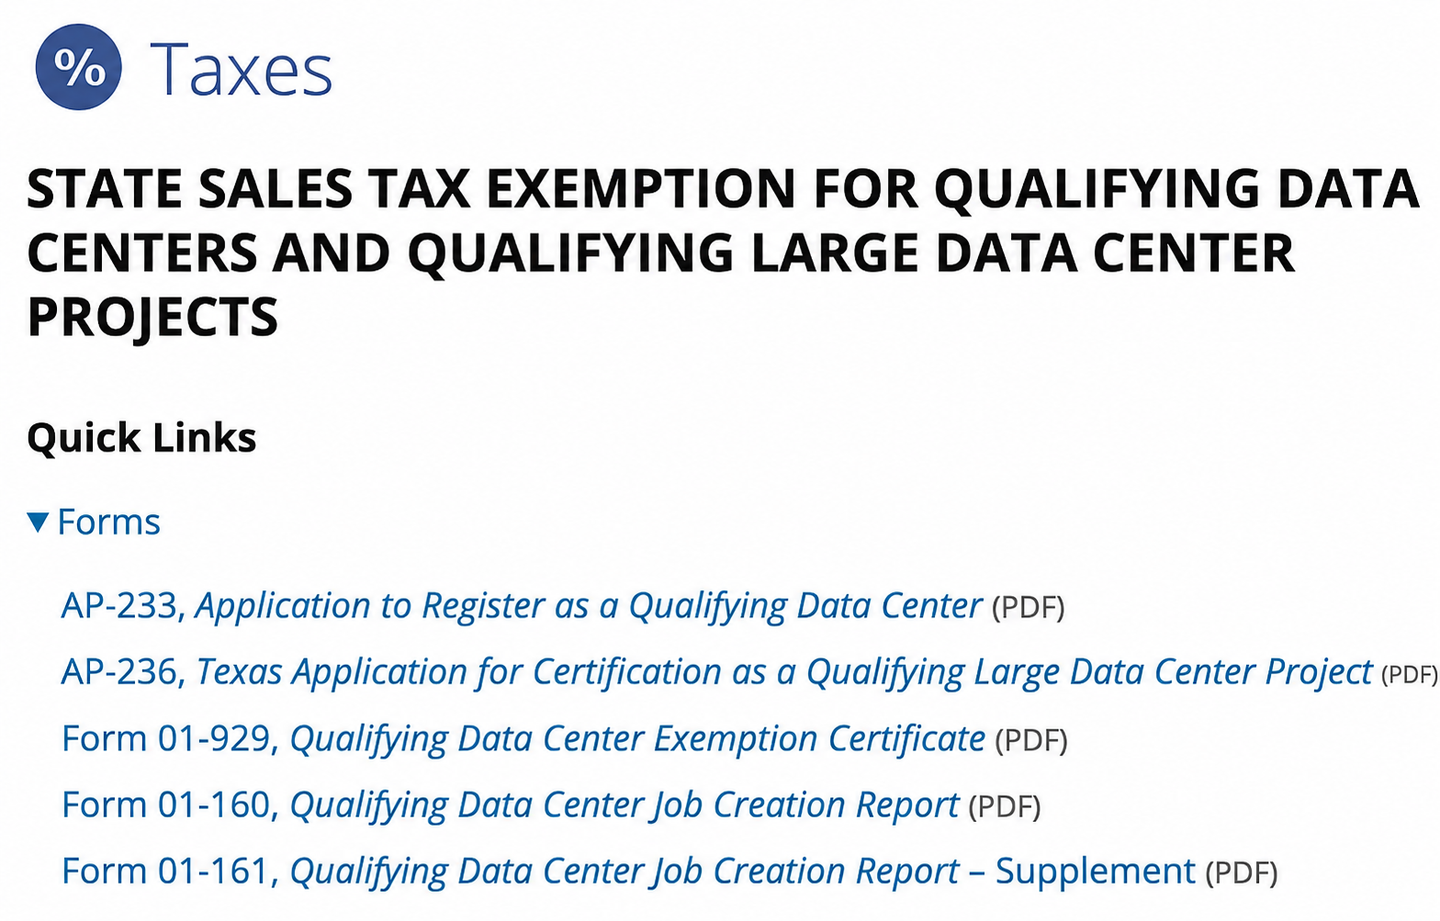
\includegraphics[width=0.48\linewidth,height=0.34\textheight,keepaspectratio]{assets/figure-5.png}\hfill
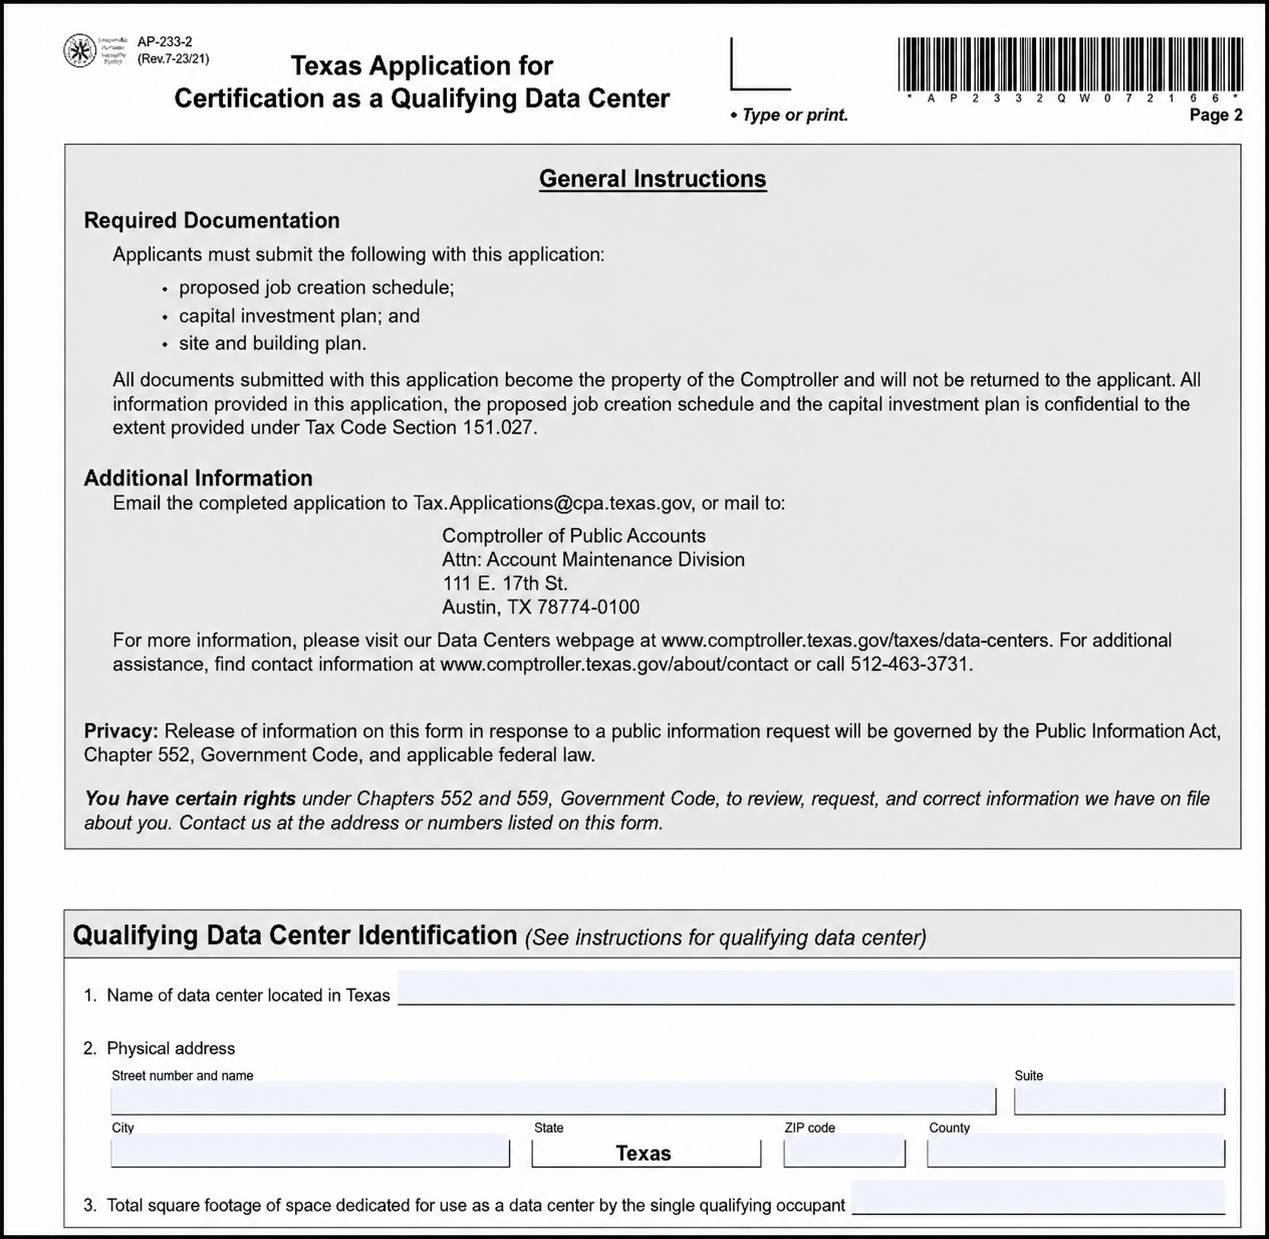
\includegraphics[width=0.48\linewidth,height=0.34\textheight,keepaspectratio]{assets/figure-6.png}
\caption{得克萨斯州合资格数据中心申请表下载页面（原文图2、图3；保留英文截图）}
\end{figure}

申请表下载：

\url{https://comptroller.texas.gov/taxes/data-centers}

\FloatBarrier
\subsection{弗吉尼亚州}

申请 DCRSUT 豁免时，符合条件的数据中心必须与弗吉尼亚州经济发展合作署（VEDP）协商并签署谅解备忘录（MOU）。VEDP 将备忘录提交州税务部门审查；获批后，税务部门直接向数据中心签发免税证书。

托管数据中心的租户须另行与数据中心签署参与证书及协议。VEDP 与州税务部门审查相关参与证书及协议后，税务部门直接向租户签发单独的免税证书。

谅解备忘录下载：

\url{https://www.vedp.org/incentive/data-center-retail-sales-use-tax-exemption}

\subsection{佐治亚州}

数据中心所有者或高科技数据中心客户，可通过佐治亚州税务中心（GTC）提交免税证书申请。在相应数据中心所有者取得免税证书之前，税务部门不会向客户签发证书。

申请过程中，数据中心可能需要提供申请人在佐治亚州的所得税申报和缴纳记录、申请人对该州不动产拥有的产权或权益价值、足以证明其可能满足高科技数据中心最低投资门槛的文件，以及其他支持材料。高科技数据中心客户还可能需要提交数据中心服务合同副本等文件。

申请说明：

\url{https://dor.georgia.gov/how-apply-high-technology-data-center-exemption}

\FloatBarrier

\section{结论}

加密矿企转型 AI 数据中心，本质上是一场“算力迁移”。在这场迁移中，税收政策是影响项目选址、投资时点和商业模式设计的重要变量之一。

矿企需要考虑的不仅是哪个州提供的优惠最多，还要评估项目能否取得优惠资格、优惠可以持续多久，以及取得资格后能否持续满足投资、就业、报告和记录保存要求。申请过晚，或在取得所需免税认证之前进行采购，可能使本可获得的节税收益落空。后续运营中未能履行绩效承诺，可能导致补缴税款、支付利息，甚至失去优惠资格。

美国各州对数据中心的政策态度正处于微妙的转折点。一些辖区继续提供力度较大的税收优惠，另一些则暂停新项目审批或缩小既有优惠范围。随着政策窗口收窄，“先行动、后申请”的做法正变得越来越难以奏效。对于计划转型的加密矿企，税收优惠申请及长期税务规划需要与投资决策同步推进。

\FloatBarrier

\section*{来源与版本说明}
\phantomsection
\addcontentsline{toc}{section}{来源与版本说明}
\noindent\textbf{英文原文。}FinTax，\textit{Crypto Miners Pivot to AI Data Centers:
U.S. State Tax Incentives and Key Considerations}，发表于\ReportDate。\par
\medskip
\noindent\href{\ReportURL}{FinTax 官网英文报告}\par
\medskip
\noindent\textbf{中文版本。}本稿于2026年11月5日依据现有英文工程翻译，为待审校的中文排版初稿，尚未与官网中文原稿核对。政策论述沿用原报告发表时的语境，未另行更新或独立核实法规。\par
\medskip
\noindent 三张表格已翻译并重排为可编辑的黑白线框表格，保留原文数值和条件。表2对两类数据中心相同的共同要求仅列示一次，并明确适用于两类项目。地图及申请表截图保留英文原图；最后两张截图合并在同一图版。第四节的申请链接沿用原文。本版本未增加额外法律分析。

% Reserved for future verified citations; the source article has no bibliography.
% \bibliographystyle{plainnat}
% \bibliography{references}
\end{document}
